\subsection{Where ShiftWM reaches the goal}
Figures~\ref{fig:qual-positive-one} and~\ref{fig:qual-positive-two} show
\emph{all four} policy-eligible development tasks on which ShiftWM (ours)
succeeds and Framewise fails. Shared context also fails on each. These are
outcome-selected explanations, not four independent benchmark improvements:
the complete eligible development comparison has one ShiftWM-only and one
Framewise-only success on PushT, and three versus eight on Reacher.
Counterexamples follow, and the local gallery retains every task.

The dashed goal silhouette makes the physical objective visible in each
observation. Both middle-column images are recorded at native call~20;
terminal images retain their actual stopping times. Reacher details use the
same crop within each case for every goal, time, and method, containing all
displayed arm poses with padding and marked in a full-scene overview.
Endpoint errors explain
why an execution satisfies or misses the scoring rule. This supports a
behavioral explanation---reaching the requested block/pusher or joint
configuration within the budget. It does not identify the responsible
internal component. Attribution to useful dynamics context, factorization,
or improved candidate ranking requires controlled interventions; the
objective/context study in Appendix~\ref{sec:rollout-revision} tests part
of this question separately.

\begin{figure}[p]
\centering
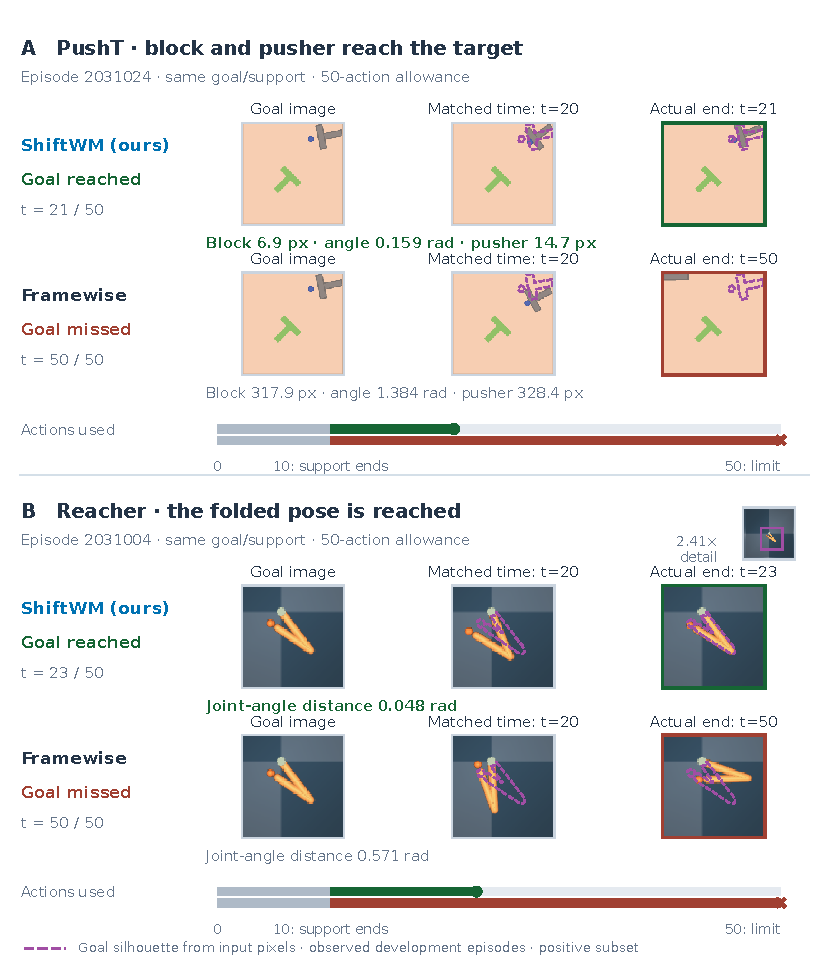
\includegraphics[width=\linewidth]{generated/qualitative/positive_1.pdf}
\caption{\textbf{Positive executions made visible: reaching the requested configuration.}
A: ShiftWM (ours) reaches the PushT block--pusher target at call~21; Framewise
continues to call~50 and moves most of the block outside the view. The recorded
terminal block/pusher errors are 6.9/14.7 versus 317.9/328.4 native pixels.
B: ShiftWM attains the folded Reacher pose at call~23; Framewise ends with a
different link orientation at call~50. Dashed purple outlines are extracted
from the common goal pixels for display only; they are not predictions or
scoring inputs. PushT's gray block and blue pusher define the requested
configuration; the green T is an unscored persistent renderer marker.
The rulers count native actions within the common allowance, including ten
support actions. Both methods face the same goal and recorded initial support.}
\label{fig:qual-positive-one}
\end{figure}

\begin{figure}[p]
\centering
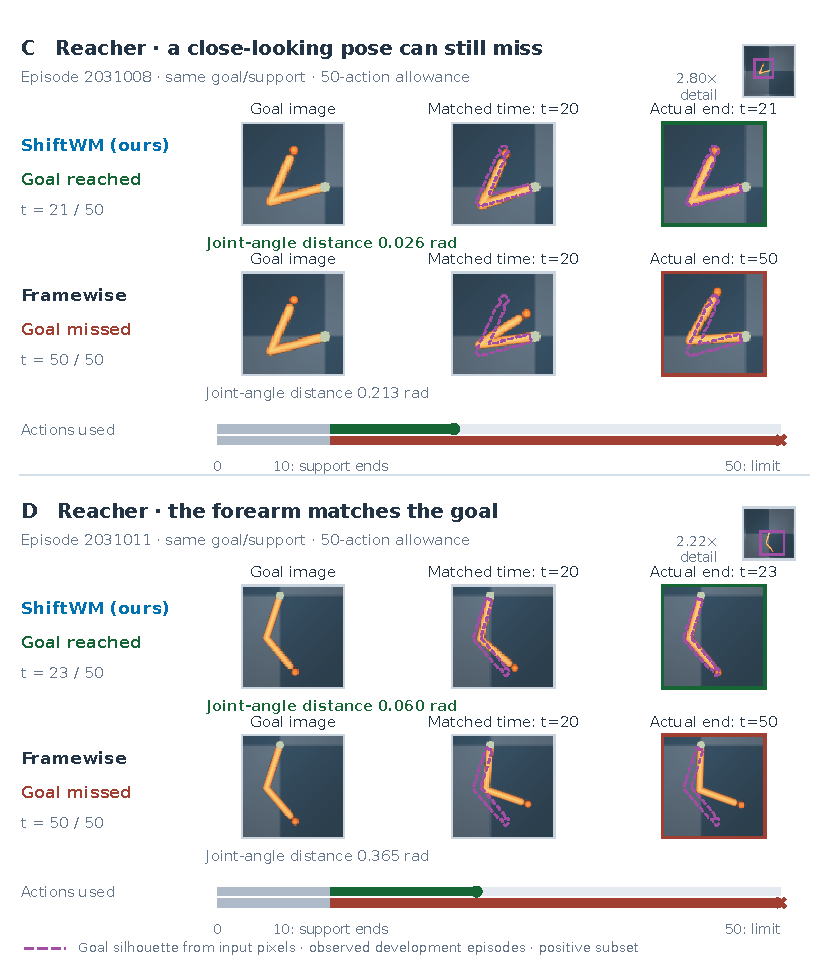
\includegraphics[width=\linewidth]{generated/qualitative/positive_2.pdf}
\caption{\textbf{Two further positive Reacher cases: goal-pose agreement matters.}
C: Framewise's final arm looks close to the goal, but retains a scored joint
mismatch; the terminal joint-angle distances are 0.026 radians for ShiftWM
(ours) and 0.213 for Framewise. D: the goal outline exposes the residual
forearm-orientation mismatch, with distances 0.060 and 0.365 radians.
ShiftWM succeeds at calls~21 and~23; Framewise fails after~50 in both cases.
Success requires each unwrapped joint error below $0.05$ radians, not an L2
distance below $0.05$; case~D therefore legitimately succeeds with $\mathrm{L2}=0.060$.
Both methods' middle frames are recorded at call~20; endpoint frames retain
their respective stopping times. Together with Figure~\ref{fig:qual-positive-one},
these exhaust the four positive discordant cases against Framewise in the
saved development comparison; Shared context also fails on all four tasks.}
\label{fig:qual-positive-two}
\end{figure}
\FloatBarrier
